\chapter{Results and Discussion}\label{results-and-discussion}

\section{Scalability Improvements}\label{results-and-discussion:s:scalability-improvements}

\subsection{Cost Rundown}\label{results-and-discussion:ss:cost-rundown}

The Infrastructure used to provide the Application to the Client is not free. As such, before comparing the older and newer architectures, the costs associated with each individual item are presented in \Cref{tab:individual-cost-aws-old} and \Cref{tab:individual-cost-aws-new}, respectively. 


\begin{table}[!htbp]
  
  \label{tab:individual-cost-aws-old}
  \resizebox{\textwidth}{!}{%
  \begin{tabular}{llccc}
  \hline
  \rowcolor[HTML]{EFEFEF} 
  Name               & Description                                                                   & \multicolumn{1}{l}{\cellcolor[HTML]{EFEFEF}\begin{tabular}[c]{@{}l@{}}Monthly\\ Use\\ (h)\end{tabular}} & \multicolumn{1}{l}{\cellcolor[HTML]{EFEFEF}\begin{tabular}[c]{@{}l@{}}Hourly\\ Cost\\ (\$/h)\end{tabular}} & \multicolumn{1}{l}{\cellcolor[HTML]{EFEFEF}\begin{tabular}[c]{@{}l@{}}Monthly\\ Cost\\ (\$/month)\end{tabular}} \\ \hline
  AWS EC2 t3a.large  & \begin{tabular}[c]{@{}l@{}}EC2 Instance with 2 vCPU and 8 GB RAM\end{tabular}      & 720                                                                                                   & 0.085                                                                                                    & 61.200                                                                                                        \\ \hline
  AWS EC2 t3a.xlarge & \begin{tabular}[c]{@{}l@{}}EC2 Instance with 4 vCPU with 16 GB RAM\end{tabular}     & 720                                                                                                   & 0.1699                                                                                                   & 122.328                                                                                                       \\ \hline
  AWS EBS Volume     & \begin{tabular}[c]{@{}l@{}}EBS Volume of type: gp2 with Size: 256 GB\end{tabular} & -                                                                                                     & -                                                                                                        & 29.696                                                                                                        \\ \hline
  \end{tabular}%
  }
  \caption{Individual Cost of AWS Infrastructure used with the old architecture. Each Month corresponds to 30 days.}
  \end{table}

Each Client using the old architecture would require one of the two \gls{ec2} instances presented in the \Cref{tab:individual-cost-aws-old} table, plus an \gls{ebs} volume. The total expenditure with infrastructure, on a monthly basis, for a Client, is the sum of the \gls{ec2} instance and the \gls{ebs} volume. Together, that value varies between \$90.896 and \$152.024. This value can be even higher, if the Client has an abnormal need for extra compute or memory resources, which would further reduce the scalability of this old architecture.

\begin{table}[!htbp]
    \caption{Individual Cost of AWS ECS Fargate Containers used in the new architecture. Each Month corresponds to 30 days.}
    \label{tab:individual-cost-aws-new}
    \resizebox{\textwidth}{!}{%
    \begin{tabular}{ccccccc}
    \hline
    \rowcolor[HTML]{EFEFEF} 
    Type                & Name and Description                                                                                          & Configuration & \begin{tabular}[c]{@{}c@{}}Daily\\ Use\\  (h)\end{tabular} & \begin{tabular}[c]{@{}c@{}}Monthly\\ Use\\ (h)\end{tabular} & \begin{tabular}[c]{@{}c@{}}Hourly\\ Cost \\ (\$/h)\end{tabular} & \begin{tabular}[c]{@{}c@{}}Monthly\\ Cost\\ (\$/month)\end{tabular} \\ \hline
                        &                                                                                                               & 0.25 vCPU     & 24                                                         & 720                                                         & 0.01215                                                         & 8.748                                                               \\ \cline{3-7} 
    \multirow{-2}{*}{A} & \multirow{-2}{*}{\begin{tabular}[c]{@{}c@{}}ECS Fargate Container\\ Very Low Power Requirements\end{tabular}} & 0.5 GB RAM    & 24                                                         & 720                                                         & 0.00265                                                         & 1.908                                                               \\ \hline
                        &                                                                                                               & 0.5 vCPU      & 24                                                         & 720                                                         & 0.02430                                                         & 17.496                                                              \\ \cline{3-7} 
    \multirow{-2}{*}{B} & \multirow{-2}{*}{\begin{tabular}[c]{@{}c@{}}ECS Fargate Container\\ Low Power Requirements\end{tabular}}      & 1 GB RAM      & 24                                                         & 720                                                         & 0.00530                                                         & 3.816                                                               \\ \hline
                        &                                                                                                               & 2 vCPU        & 0.25                                                       & 7.5                                                         & 0.09720                                                         & 0.729                                                               \\ \cline{3-7} 
    \multirow{-2}{*}{C} & \multirow{-2}{*}{\begin{tabular}[c]{@{}c@{}}AWS Fargate Container\\ Medium Power Requirements\end{tabular}}   & 4 GB RAM      & 0.25                                                       & 7.5                                                         & 0.02120                                                         & 0.159                                                               \\ \hline
                        &                                                                                                               & 2 vCPU        & 0.5                                                        & 15                                                          & 0.09720                                                         & 1.458                                                               \\ \cline{3-7} 
    \multirow{-2}{*}{D} & \multirow{-2}{*}{\begin{tabular}[c]{@{}c@{}}AWS Fargate Container\\ Medium Power Requirements\end{tabular}}   & 4 GB RAM      & 0.5                                                        & 15                                                          & 0.02120                                                         & 0.318                                                               \\ \hline
                        &                                                                                                               & 4 vCPU        & 1.50                                                       & 45                                                          & 0.19440                                                         & 8.748                                                               \\ \cline{3-7} 
    \multirow{-2}{*}{E} & \multirow{-2}{*}{\begin{tabular}[c]{@{}c@{}}AWS Fargate Container\\ High Power Requirements\end{tabular}}     & 8 GB RAM      & 1.50                                                       & 45                                                          & 0.04240                                                         & 1.908                                                               \\ \hline
    \end{tabular}%
    }
    \end{table}

\begin{figure}[!htbp]
    \centering
    \fbox{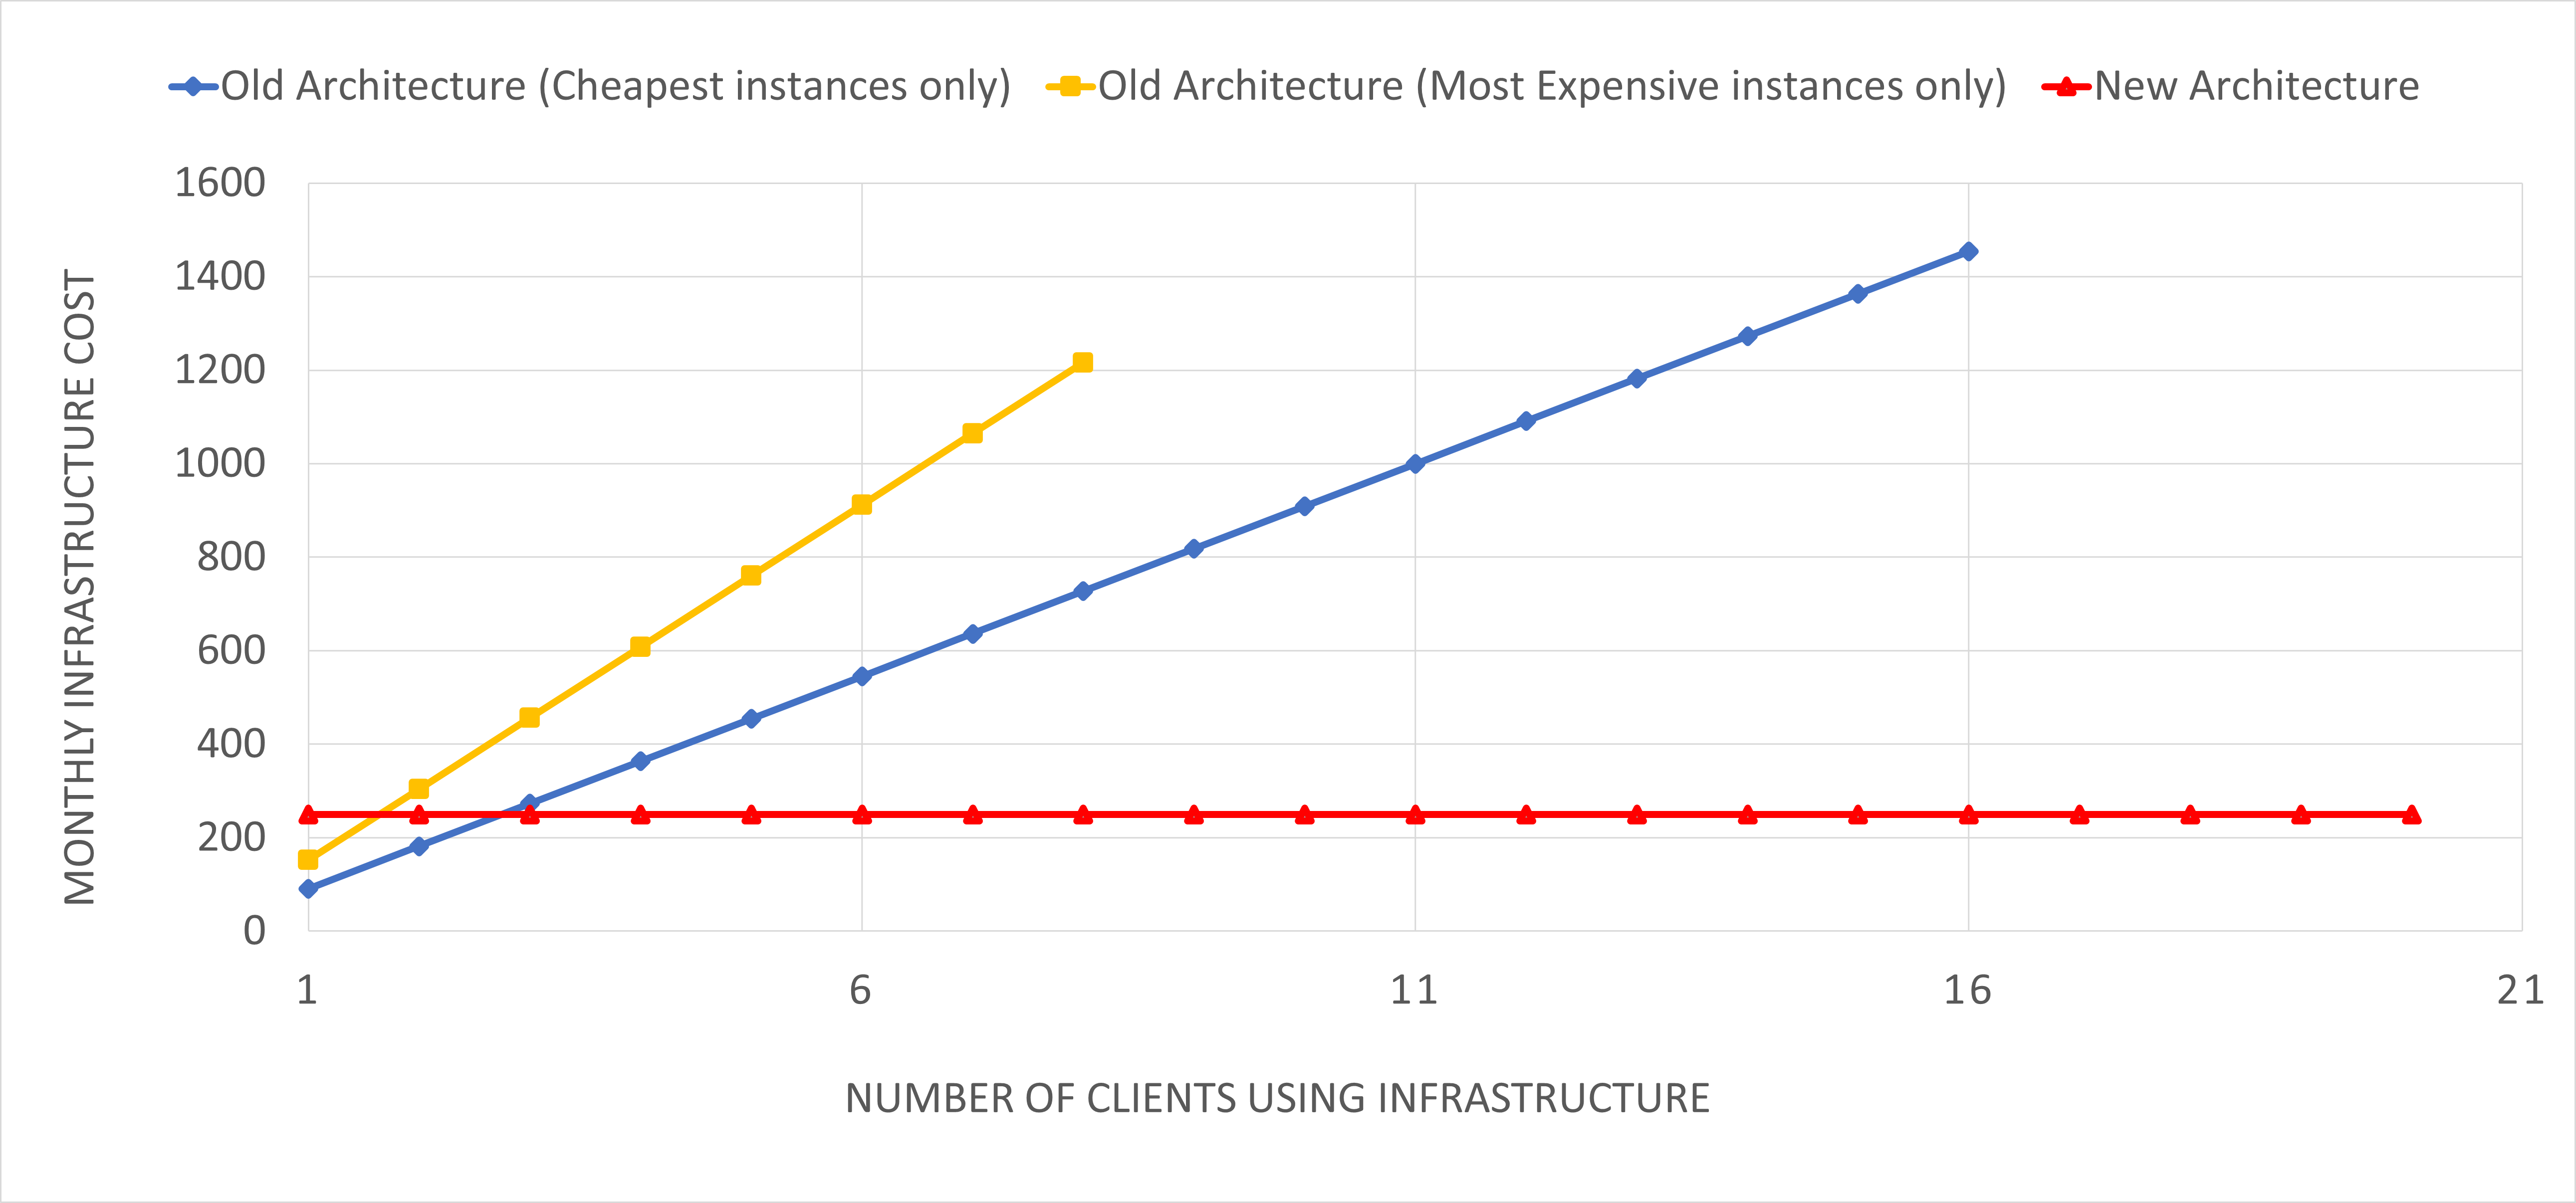
\includegraphics[width=0.95\textwidth]{img/charts/infra-cost-per-client.png}}
    \caption[Infrastructure Cost Per Client]{Infrastructure Cost Per Client.}
    \label{fig:infra-cost-per-client}
\end{figure} 
    

As mentioned in \cref{methodology:sss:scaling}, due to constraints in the AWS EC2 service, there is a maximum limit of 32 \gls{vcpu} units for each AWS account. This means that, even if all of the Clients only required the smaller option that uses 2 \gls{vcpu}, the maximum number of Clients would still be only 16 Clients. With the new architecture, there is no hard limit on the number of clients that can be served simultaneously. As of the time of writing, the new architecture is currently serving three different clients, being that one of these Clients has a water network that generates as much data as all previous Clients combined, for both the old architecture and the new one. It was also tested using 17 fictional Clients, totaling 20 Clients being served by the Application simultaneously, with no discernible issues for the Users nor resource usages above the normal everyday operation with the three regular Clients.

The new architecture has one Application for each development environment --- Production, Staging and Internal. Using \Cref{tab:individual-cost-aws-new} as reference, each Environment uses two containers of type A for the PostgreSQL database and Redis services, two containers of type B for Backend API and InfluxDB database services, one container of type C and D for the Forecasting and KPI Calculation services, respectively. Finally, type E containers are used for the Optimization service. In order to test reducing even further the resource usage for services that are running constantly, in the Internal environment, the Backend API service and InfluxDB database service have been scaled down vertically to use containers of type A. Additionally, other services are being run in this Internal environment for further testing, but are not accounted here due to being temporary services used while the Web Platform is not ready for Production.



As can be observed in \cref{fig:infra-cost-per-client}, the monthly cost of maintaining the infrastructure needed for the Application scales linearly for the old architecture, while the new architecture's cost for low amounts of Clients is kept steady. Despite the fact that the new infrastructure has not yet been tested for more than 20 Clients, hence the data in the figure ending at 20 clients, according to the resource usage during both peak hours and idle times, these were largely unaltered, and usage difference was negligible. Therefore, the usage of the Application using the new architecture is sure to be capable of handling many more Clients simultaneously.


\subsubsection{Remaining Costs}\label{results-and-discussion:sss:remaining-costs}

The costs presented here are only the main costs associated with the differences between the architectures. These are the bulk of the monthly costs with the infrastructure used.
There are also costs related to Data Transfer in and out of the \gls{vpc}, costs with Costumer Support, costs associated with automatic backups of data and other resources. Some resource usages are not reported in this document due to Client confidentiality agreements, being free of charge or being used so sparingly or in low quantities that the costs are irrelevant or included in the Free Tier\footnote{Certain AWS resources are free until a certain level of usage is achieved.}.

\subsection{Development and Deployment Issues}\label{results-and-discussion:ss:development-and-deployment-issues}

Besides the infrastructural scaling issue, there was also a problem scaling the human resources needed for development. Having the Application be the same for all of the Clients, instead of being one separately maintained Application for each Client, drastically lowers the developer manpower needed for maintaining and updating an Application for multiple Clients. Therefore, this new architecture is substantially and clearly scalable when compared with the previous architecture.

\section{DevOps Improvements}\label{results-and-discussion:s:devops-improvements}

The Company's developer team's general sentiment towards the implementation of the new architecture is one of relief and excitement. As stated in \Cref{methodology:sss:deployments} and \cref{methodology:sss:testing}, there were several issues regarding the developer workflow when working in the Application. After implementing the new architecture, these concerns have diminished considerably. The measures taken in \cref{methodology:ss:solving-the-deployment-issues} and \Cref{methodology:sss:testing-new} have brought a new and better workflow to the development team. This can be attested by the results in the \gls{fkm}.

\subsection{Deployment Frequency}\label{results-and-discussion:ss:deployment}

In order to measure the deployment frequency of the old architecture, GitLab's tagging list for a select number of Clients was analyzed. As stated in \Cref{methodology:sss:deployments}, each deployment made to the old architecture's infrastructure was linked to a \textit{tag} in the subversion control system. Following the history for each tag since the first day of January 2020, ignoring failures to deploy due to badly configured CI/CD elements, the table present in \cref{tab:old-deployments-per-quarter} was elaborated. Client's names are omitted due to confidentiality agreements. Client C****'s Application was only pushed into Production on the 11th of April 2021, hence the lack of data up until the 2nd quarter of that year. Despite the fact that the deployments made for these older clients were made due to updates or bugs in different modules of the Application, since the Application has very high deployment coupling, the process of deployment was nearly identical for all of these events and counted towards this table in the same manner.

\begin{table}[!htbp]
    \caption{Number of Deployments per Yearly Quarter for three Clients using the old Application.}
\label{tab:old-deployments-per-quarter}
\resizebox{\textwidth}{!}{%
\begin{tabular}{cccccc}
\hline
\rowcolor[HTML]{EFEFEF} 
Year                   & Quarter & Client A*** & Client C**** & Client I**** & Total Number of Deployments \\ \hline
                        & 1st     & 2           & -            & 5            & 7                           \\ \cline{2-6} 
                        & 2nd     & 1           & -            & 2            & 3                           \\ \cline{2-6} 
                        & 3rd     & 1           & -            & 3            & 4                           \\ \cline{2-6} 
\multirow{-4}{*}{2020} & 4th     & 9           & -            & 2            & 11                          \\ \hline
                        & 1st     & 18          & -            & 3            & 21                          \\ \cline{2-6} 
                        & 2nd     & 2           & 11           & 0            & 13                          \\ \cline{2-6} 
                        & 3rd     & 3           & 9            & 0            & 12                          \\ \cline{2-6} 
\multirow{-4}{*}{2021} & 4th     & 0           & 1            & 0            & 1                           \\ \hline
                        & 1st     & 0           & 0            & 0            & 0                           \\ \cline{2-6} 
\multirow{-2}{*}{2022} & 2nd     & 0           & 0            & 1            & 1                           \\ \hline
\end{tabular}%
}

\end{table}

The choice of the time period was done purposely for several reasons. The first is related to the recent SARS-Cov2 pandemic that changed the workflow inside the Company, seeing that the workforce was relocated to working-from-home during the year of 2020. The second reason was the development team itself, that changed considerably during the pandemic. Third reason was the influence of this project to build a new architecture, since it changed the Company's development priorities. The idea of a new architecture was considered somewhere in 2020, and became a priority in late 2021. The development and deployment of updates to Clients is not uniformly distributed throughout this time period, since newer Clients become priority as the amount of work is greater at the beginning of a new Client project. The table is indexed by time, with time periods of 4 months, in order not to occupy too much space in the document. For each block of 4 months, it's presented the total number of deployments performed for each Client during that time period. 

From \Cref{tab:old-deployments-per-quarter}, it also becomes apparent that the development team does not work on multiple projects simultaneously with the same involvement. Each time a Client requires refactoring or updates, the amount of deployments performed to other clients drops drastically. It can also be observed that, unless a refactor or big update is required, the amount of deployments is very reduced or non-existent.
Finally, the plan to move these older Clients to the new Application that uses the new architecture is being put into place and the updates to the old Applications was put on hold, to focus work on the new architecture. This fact reflects on the lack of deployments for these older Clients since the fourth quarter of 2021, when the project to migrate to the new Application was started.

\begin{table}[!htbp]
\caption{Number of monthly deployment events per service in the new architecture. Data collected from March 3rd to June 23rd, 2022.}
\label{tab:new-service-deployments-monthly}
\resizebox{\textwidth}{!}{%
\begin{tabular}{ccccccccc}
\hline
\rowcolor[HTML]{EFEFEF} 
Month & \begin{tabular}[c]{@{}c@{}}Backend\\ API\end{tabular} & InfluxDB & PostgreSQL & \begin{tabular}[c]{@{}c@{}}Forecast\\ Worker\end{tabular} & \begin{tabular}[c]{@{}c@{}}Optimization\\ Worker\end{tabular} & \begin{tabular}[c]{@{}c@{}}Perfomance\\ Worker\end{tabular} & Redis & Total \\ \hline
March & 5                                                     & 2        & 2          & 4                                                         & -                                                             & 2                                                           & 2     & 17    \\ \hline
April & 5                                                     & 0        & 0          & 0                                                         & 5                                                             & 2                                                           & 0     & 12    \\ \hline
May   & 2                                                     & 0        & 0          & 0                                                         & 11                                                            & 0                                                           & 0     & 13    \\ \hline
June  & 3                                                     & 0        & 0          & 2                                                         & 1                                                             & 1                                                           & 0     & 7     \\ \hline
\end{tabular}%
}

\end{table}

As for the Deployment Frequency of the new architecture and the new Application, the measurement was performed differently. Since each service is deployed independently, \Cref{tab:new-service-deployments-monthly} gathers the number of deployment per service per time period. Preparing the old architecture's components to accept multiple users and study, implement and test each one of them took some time, the deployment of the new architecture is relatively recent. Therefore, the time periods used in the table are in monthly intervals.

Although there are only 4 months of available data, a trend can be seen. In comparison with the old architecture, the amount of total deployments per month has increased, increasing the Deployment Frequency.

\subsection{Lead Time for Change}\label{results-and-discussion:ss:lead-time-for-change}

Lead time for change, as a result of the new architecture and the new workflow it brings to the Company, has decreased rapidly. Whereas changes would take hours or even days to reach Production in the old architecture, the new architecture is able to deploy a new version of a service in a matter of minutes. There is no table for this subsection of results for multiple reasons:
Firstly, because the planned Observability platform is not yet ready nor are the automatic \gls{cicd} procedures currently running. Due to this, data cannot be reliably obtained from neither an automatic Observability platform nor from a local registry. The development team is small and since the new architecture is still not finished, deployments have been made manually and, for that reason, there are no reliable records of when those deployments occurred. 

Although this value cannot be stated, it can be empirically seen that this metric has decreased, which is an improvement. During the development of this implementation of the new architecture, there were only two persons working full time on this. Assuming the amount of re-prioritizing tasks was minimal, each developer mostly only addressed a change at a time. This means that every deployment was the result of the most recent change to code. Empirically, since the deployment and implementation coupling is low or non-existent, changes made to code were put into Production as soon as possible, leaving minutes or hours between changes and their deployment to Production. This was exacerbated since there were no real Clients using the new Application until the last month, July 2022, so the failure of a component was not a critical issue.

Therefore, it can be considered that the Lead Time for Change has improved.

\subsection{Time to Restore Service}\label{results-and-discussion:ss:Time to Restore Service}

Likewise, the fact that the new architecture possesses low-to-nonexistent deployment coupling made the Time to Restore Service reach lower values. This can be seen by the fact that it is no longer required to deploy the whole Application in order to publish a fix to Production. There are also no \gls{ec2} instances to be restarted, so this time is even shorter now. Once again, however, this cannot be observed directly and objectively since there is no numerical data to back up this claim in a mathematical way.

\subsection{Change Failure Rate}\label{results-and-discussion:ss:change-failure-rate}

As previously referred in \cref{methodology:ss:solving-the-deployment-issues}, the new architecture's ability to test the code multiple times in similar environments drastically reduces the Change Failure Rate. This cannot be measured yet, for multiple reasons. Firstly, like the other metrics, there are no Observability metrics for this metric. Secondly, since this new architecture project is still being developed actively, the amount of changes is higher than would be expected during a normal time and so, this number should not be taken into account.
Nevertheless, the changes to the architecture should prove that this metric has improved as soon as more data is available.


\section{Observability Improvements}\label{results-and-discussion:ss:observability-improvements}

As for Observability of the System, this has increased, reaching the goal that was set out in the beginning of the project.
The old architecture has no Observability, with the exception of the logs that are aggregated by Google Cloud's operations suite, formerly Stackdriver\footnote{https://cloud.google.com/products/operations\label{foot:stackdriver}} and AWS's \gls{ec2} machine 
